\documentclass[trans]{beamer}
\usepackage{etex}
\usepackage{amsthm}
\usepackage{xcolor}
\usepackage{wrapfig}
\usepackage{soul}
\usepackage{lipsum}
\usepackage{booktabs}
\usepackage{graphicx}
\usepackage{algorithm}
\usepackage{algorithmic}
\usepackage{answers}
\usepackage[absolute,overlay]{textpos}
\usepackage{verbatim}
\usepackage{fancyvrb}
\usepackage{xspace}
%\usepackage[labelsep=none]{caption}
\usepackage{tikz}
\usepackage{units}
\usepackage{makeidx}
\usepackage{tabularx}
\usepackage{colortbl}
\usepackage{multirow}
\usepackage{calc}
%\usepackage{graphicx}
%\usepackage{array}
%\usepackage[all]{xy}
%%\usepackage{theapa}
%\usepackage{tikz}
%\usetikzlibrary{shapes.geometric} 
%\usetikzlibrary{shadows} 
%\usetikzlibrary{positioning}
%\usepackage{algorithm}
%%\usepackage{algorithmic}
%\usepackage{algorithmic}
%%\usepackage{algpseudocode}
%\usepackage{natbib}
%\usepackage{apalike}
\usepackage{../book/haldefs}

\mode<presentation>
{
%  \usetheme{AnnArbor}
%  \usetheme{Antibes}
%  \usetheme{Bergen}
%  \usetheme{Berkeley}
%  \usetheme{Berlin}
%  \usetheme{Boadilla}
%  \usetheme{boxes}
%  \usetheme{CambridgeUS}
%  \usetheme{Copenhagen}
%  \usetheme{Darmstadt}
%  \usetheme{default}
%  \usetheme{Dresden}
%  \usetheme{Frankfurt}
%  \usetheme{Goettingen}
%  \usetheme{Hannover}
%  \usetheme{Ilmenau}
%  \usetheme{JuanLesPins}
%  \usetheme{Luebeck}
%  \usetheme{Madrid}
%  \usetheme{Malmoe}
%  \usetheme{Marburg}
%  \usetheme{Montpellier}
%  \usetheme{PaloAlto}
%  \usetheme{Pittsburgh}
%  \usetheme{Rochester}
%  \usetheme{Singapore}
%  \usetheme{Szeged}
%  \usetheme{Warsaw}
  \usetheme{Unife}

%\usecolortheme{lily}% 
  % or ...

  \setbeamercovered{transparent}
  % or whatever (possibly just delete it)
}


\usepackage[english]{babel}
% or whatever

%\usepackage[latin1]{inputenc}
% or whatever
\usetikzlibrary{shapes,snakes}
%%% Local Variables: 
%%% mode: latex
%%% TeX-master: "courseml"
%%% End: 

%%%%%%%%%%% COLORS

\definecolor{darkgrey}{rgb}{0.2,0.2,0.2}
\definecolor{grey}{rgb}{0.9,0.9,0.9}
\definecolor{darkblue}{rgb}{0.0,0.0,0.5}
\definecolor{darkpurple}{rgb}{0.4,0.0,0.4}
\definecolor{darkred}{rgb}{0.5,0.0,0.0}
\definecolor{darkorange}{rgb}{0.5,0.45,0.4}
\definecolor{darkgreen}{rgb}{0.0,0.5,0.0}
\definecolor{darkergreen}{rgb}{0.0,0.4,0.0}
\definecolor{lightblue}{rgb}{0.8,0.8,1.0}
\definecolor{lightgreen}{rgb}{0.8,1.0,0.8}
\definecolor{lightred}{rgb}{1.0,0.8,0.8}
\definecolor{lightyellow}{rgb}{1.0,1.0,0.8}
\definecolor{lightorange}{rgb}{1.0,0.9,0.8}
\definecolor{lightgrey}{rgb}{0.96,0.97,0.98}

%%%%%%%%%%%%% FORMATTING

\definecolor{darkbookcolor}{rgb}{0.4,0.0,0.45} % was darkergreen
\definecolor{lightbookcolor}{rgb}{0.98,0.9,1.0} % was green!20

\newcommand*\chapterlabel{}
\makeatletter
\titleformat{\chapter}%
  [block]                                % shape
  {\gdef\chapterlabel{}
   \normalfont\sffamily\Huge\bfseries\scshape}            % format applied to label+text
  {\gdef\chapterlabel{\thechapter~|~}}    % 
  {0pt}                                  % horizontal separation between label and title body
  {\begin{tikzpicture}[remember picture,overlay]
    \node[yshift=-3cm] at (current page.north west)
      {\begin{tikzpicture}[remember picture, overlay]
        \draw[fill=lightbookcolor] (0,0) rectangle
          (\paperwidth,3cm);
        \node[anchor=east,xshift=.9\paperwidth,rectangle,
              rounded corners=20pt,inner sep=11pt,
              fill=darkbookcolor]
              {\color{white}\chapterlabel#1};
       \end{tikzpicture}
      };
   \end{tikzpicture}
  }% before the title body
  []%after the title body
\makeatother 
%\titlespacing*{\chapter}{0pt}{50pt}{-10pt}

\newcommand{\sectionsize}{}
\titleformat{\section}%
  [hang]% shape
  {\normalfont\Large\itshape}% format applied to label+text
  {\textcolor{darkbookcolor}{\makebox[0pt][r]{\thesection\quad }#1}}% label
  {1em}% horizontal separation between label and title body
  {}% before the title body
  []% after the title body

\titleformat{\subsection}%
  [hang]% shape
  {\normalfont\large\itshape}% format applied to label+text
  {\textcolor{darkbookcolor}{\makebox[0pt][r]{\thesubsection\quad }#1}}% label
  {1em}% horizontal separation between label and title body
  {}% before the title body
  []% after the title body



%%%%%%%%%%% EXERCISE STUFF

\newtheorem{Ex}{Exercise}[chapter]
\newenvironment{exercises}{\section{Exercises}}{}
% \center\begin{tabular}{c}\hline{\bf\Large Exercises}\\\hline\end{tabular}}{}

\Newassociation{solution}{Soln}{solutions}
\Newassociation{hint}{Hint}{solutions}
\newcommand{\prehint}{~[Hint]}
\newcommand{\presolution}{}
\newcommand{\Opensolutionshook}[2]%
  {\Writetofile{#1}{}}
\renewcommand{\Solnlabel}[1]{%
  {\Large\linespread{1}%
  \begin{tabular}{|p{\textwidth}@{}|}%
    \hline%
    \emph{Solution #1}\\%
    \hline%
  \end{tabular}\newline}}
\renewcommand{\Hintlabel}[1]{\emph{Hint #1}}


\newcommand{\emptylist}{[ ]}
\newcommand{\pushlist}[1]{{\ensuremath \oplus} #1}

\newcommand*\learningproblemargument{}
\newsavebox{\learningproblembox}
\newenvironment{learningproblemenv}[1]
  {\gdef\learningproblemargument{#1}\begin{lrbox}{\learningproblembox}\begin{minipage}{4in}}
  {\end{minipage}\end{lrbox}%
   \tikzstyle{mybox} = [draw=darkbookcolor, fill=lightbookcolor, very thick, rectangle, rounded corners, inner sep=10pt, inner ysep=12pt]%
   \tikzstyle{fancytitle} =[fill=darkbookcolor, text=white, rectangle, rounded corners]%
   \vspace{1em}
   \noindent
   \begin{tikzpicture}
     \node [mybox] (box) {\usebox{\learningproblembox}};
     \node [fancytitle, right=10pt] at (box.north west) {\normalfont\sffamily\Large\bfseries\scshape Task: \learningproblemargument};
   \end{tikzpicture}
  }

\newcommand{\learningproblem}[3]{
  \begin{learningproblemenv}{#1}
    \emph{Given:}
    \begin{enumerate}
      #2
    \end{enumerate}
    \emph{Compute:} #3
  \end{learningproblemenv}}

\newcommand{\lprob}[1]{{\normalfont\sffamily\scshape #1}}

%%%%%%%%%%% ENVIRONMENTS

\DefineVerbatimEnvironment%
  {chapternotes}{Verbatim}
  {baselinestretch=1.0,frame=single,fillcolor=\color{lightbookcolor}}
%\renewenvironment{chapternotes}{\begin{comment}}{\end{comment}}

\newenvironment{editedout}{\begin{comment}}{\end{comment}}

\newenvironment{derivation}
  {\begin{eqnarray}}
  {\end{eqnarray}}

\newcommand{\derivstep}[2]{#1\sidenote{#2}}

%\makeatletter\newenvironment{learninggoals}{%
%   ~\\\noindent\begin{lrbox}{\@tempboxa}\begin{shadowblock}{\columnwidth}\begin{itemize}}{\end{itemize}\end{shadowblock}\end{lrbox}%
%   {\usebox{\@tempboxa}}
%}\makeatother

%\newenvironment{learningobjectives}
%  {\begin{marginfigure}\begin{learninggoals}\item[]\item[] \hspace{-2em} {\bf Learning Objectives:}}
%  {\end{learninggoals}\end{marginfigure}}

\newsavebox{\objectivesbox}
\newlength{\objectivesheight}
\newenvironment{learningobjectives}
  {\begin{lrbox}{\objectivesbox}\begin{minipage}{2in}\vspace{2pt}{\bf Learning Objectives:}\begin{footnotesize}\begin{itemize}}
  {\end{itemize}\end{footnotesize}\end{minipage}\end{lrbox}\begin{textblock}{2}(10.2,2.5)\begin{shadowblock}{2in}\usebox{\objectivesbox}\end{shadowblock}\end{textblock}\settoheight{\objectivesheight}{\usebox{\objectivesbox}}}

\newenvironment{chapterintro}
  {}
  {}

\newcommand*\vignetteargument{}
\newsavebox{\vignettebox}
\newenvironment{vignette}[1]
  {\gdef\vignetteargument{#1}\begin{lrbox}{\vignettebox}\begin{minipage}{6.4in}}
  {\end{minipage}\end{lrbox}%
   \tikzstyle{mybox} = [draw=Periwinkle, fill=Periwinkle!5, very thick, rectangle, rounded corners, inner sep=10pt, inner ysep=12pt]%
   \tikzstyle{fancytitle} =[fill=Periwinkle, text=white, rectangle, rounded corners]%
   \vspace{1em}
   \noindent
   \begin{tikzpicture}
     \node [mybox] (box) {\usebox{\vignettebox}};
     \node [fancytitle, right=10pt] at (box.north west) {\normalfont\sffamily\Large\bfseries\scshape Vignette: \vignetteargument};
   \end{tikzpicture}
  }

%[transform shape, baseline=-3.5cm]
\newcommand*\mathreviewargument{}
\newsavebox{\mathreviewbox}
\newenvironment{mathreview}[1]
  {\gdef\mathreviewargument{#1}\begin{lrbox}{\mathreviewbox}\begin{minipage}{6.4in}}
  {\end{minipage}\end{lrbox}%
   \tikzstyle{mybox} = [draw=Sepia, fill=Sepia!5, very thick, rectangle, rounded corners, inner sep=10pt, inner ysep=12pt]%
   \tikzstyle{fancytitle} =[fill=Sepia, text=white, rectangle, rounded corners]%
   \begin{figure*}[t]
     \begin{tikzpicture}
       \node [mybox] (box) {\usebox{\mathreviewbox}};
       \node [fancytitle, right=10pt] at (box.north west) {\normalfont\sffamily\Large\bfseries\scshape Math Review | \mathreviewargument};
     \end{tikzpicture}
     %\caption[Math Review: \mathreviewargument]{~}
   \end{figure*}%
  }


%\newenvironment{chapterquote}
%  {\textblockcolor{grey}\begin{textblock}{6.5}(8,1)}
%  {\end{textblock}}

%\newenvironment{chapterimage}
%  {\textblockcolor{white}\begin{textblock}{6.5}(8,1)}
%  {\end{textblock}}


%  {\par\linespread{1}\center%
%   \begin{greybox}%
%   \begin{tabular}{|p{4in}|}%
%     \hline\vspace{+0.02in}%
%     \rule{1ex}{1ex} Learning Goals \rule{1ex}{1ex}%
%     }
%  { \vspace{+0.05in}\\\hline%
%   \end{tabular}\vspace{+0.1in}\end{greybox}\\}\makeatother


%%%%%%%%%%% COMMANDS

\newcommand{\bigemph}[1]{\textcolor{darkblue}{\bf #1}}

\newcommand{\dependencies}[1]{\marginnote[2.5in]{Dependencies: #1}}

%\newcommand{\dependencies}[1]{\begin{textblock}{2}(10.2,2.5)Dependencies: #1\end{textblock}}

\sethlcolor{lightyellow}

\newcommand{\concept}[1]{\hl{\bf #1}\index{#1}}
\newcommand{\koncept}[2]{\hl{\bf #1}\index{#2}}

\newcommand{\chref}[1]{Chapter~\ref{#1}}


\newcommand{\chapterquote}[2]
  {\tikzstyle{mybox} = [draw=darkbookcolor, fill=lightbookcolor, very thick, rectangle, rounded corners, inner sep=5pt, inner ysep=5pt]
   \tikzstyle{fancytitle} =[fill=darkbookcolor, text=white]
   \begin{textblock}{7.5}(2,2.5)
   \begin{tikzpicture}[transform shape, rotate=0, baseline=-3.5cm]
   \noindent%
   \node [mybox] (box) {%
    \begin{minipage}[t!]{\textwidth}
      \noindent%
      \begin{large}%
      \textsf{#1}%
      \end{large}
      \hfill\textcolor{darkbookcolor}{\textsf{--~#2}}
    \end{minipage}
    };
%   \node[fancytitle] at (box.south) {\emph{-- #2}};
  \end{tikzpicture}
  \end{textblock}}

\newcommand{\chapterimage}[2]
  {\tikzstyle{mybox} = [draw=darkbookcolor, fill=lightbookcolor, very thick, rectangle, rounded corners, inner sep=5pt, inner ysep=5pt]
   \tikzstyle{fancytitle} =[fill=darkbookcolor, text=white]
   \begin{textblock}{7.5}(2,2.5)
   \begin{tikzpicture}[transform shape, rotate=0, baseline=-3.5cm]
   \noindent
   \node [mybox] (box) {%
    \begin{minipage}[t!]{\textwidth}
      \includegraphics[width=\textwidth]{#1}

      \hfill\textcolor{darkbookcolor}{\textsf{--~#2}}
    \end{minipage}
    };
%   \node[fancytitle] at (box.south) {\emph{-- #2}};
  \end{tikzpicture}
  \end{textblock}}

\newcommand{\chapterimageopt}[3]
  {\tikzstyle{mybox} = [draw=darkbookcolor, fill=lightbookcolor, very thick, rectangle, rounded corners, inner sep=5pt, inner ysep=5pt]
   \tikzstyle{fancytitle} =[fill=darkbookcolor, text=white]
   \begin{textblock}{7.5}(2,2.5)
   \begin{tikzpicture}[transform shape, rotate=0, baseline=-3.5cm]
   \noindent
   \node [mybox] (box) {%
    \begin{minipage}[t!]{\textwidth}
      \includegraphics[#2]{#1}

      \hfill\textcolor{darkbookcolor}{\textsf{--~#3}}
    \end{minipage}
    };
%   \node[fancytitle] at (box.south) {\emph{-- #2}};
  \end{tikzpicture}
  \end{textblock}}


\newcommand{\monthyear}{%
  \ifcase\month\or January\or February\or March\or April\or May\or June\or
  July\or August\or September\or October\or November\or
  December\fi\space\number\year
}

\newcommand{\blankpage}{\newpage\hbox{}\thispagestyle{empty}\newpage}
\newcommand{\mycite}[1]{\sidenote{\citealt{#1}}}
\newcommand{\bookurl}{\url{http://ciml.info/}}

\newcommand{\TODOFigure}[2]{%
  \begin{marginfigure}
    \framebox[\textwidth][c]{\begin{minipage}{\textwidth}\rule{0pt}{2in}\end{minipage}}
    \caption{{\tt #1}: #2}
    \label{fig:#1}
  \end{marginfigure}}

\newlength{\NextFigureOffset}
\newcommand{\ResetNextFigure}{\setlength{\NextFigureOffset}{0mm}}
\newcommand{\MoveNextFigure}[1]{\setlength{\NextFigureOffset}{#1}}

\ResetNextFigure{}

\newcommand{\Figure}[2]{%
  \begin{marginfigure}[\NextFigureOffset]
    \begin{centering}
    \includegraphics[width=\textwidth]{figs/#1}
    \caption{#2}
    \label{fig:#1}
    \end{centering}
  \end{marginfigure}
  \ResetNextFigure{}
  }

\newcommand{\FigureFull}[2]{%
  \begin{figure}
    \begin{centering}
    \includegraphics[width=\textwidth]{figs/#1}
    \caption{#2}
    \label{fig:#1}
    \end{centering}
  \end{figure}
  }

\newcommand{\Table}[4]{%
  \begin{margintable}
    \begin{centering}
    \begin{tabular}{#3}
      #4
    \end{tabular}
    \caption{#2}
    \label{tab:#1}
    \end{centering}
  \end{margintable}}

\newcommand{\TableSize}[5]{%
  \begin{margintable}
    \begin{centering}
    \begin{#1}
    \begin{tabular}{#4}
      #5
    \end{tabular}
    \caption{#3}
    \label{tab:#2}
    \end{#1}
    \end{centering}
  \end{margintable}}

\newcommand{\thinkaboutit}[1]{%
\marginnote{
   \noindent
  \begin{tikzpicture}[transform shape, rotate=0, baseline=-1cm]
   \node [draw=Blue, fill=Blue!10, very thick, rectangle, rounded corners, inner sep=8pt, inner ysep=5pt] (box) {%
    \begin{minipage}[t!]{1.8in}
      #1
    \end{minipage}
    };
   \node[fill=Blue, text=white] at (box.west) {\textsf{\LARGE ?}};
  \end{tikzpicture}
}
}

\newenvironment{myproof}[1]%
  {\begin{proof}[Proof of Theorem~#1]}
  {\end{proof}}

\definecolor{gray0.00}{rgb}{1,1,1}
\definecolor{gray0.20}{rgb}{0.9,0.9,0.9}
\definecolor{gray0.26}{rgb}{0.87,0.87,0.87}
\definecolor{gray0.30}{rgb}{0.85,0.85,0.85}
\definecolor{gray0.32}{rgb}{0.84,0.84,0.84}
\definecolor{gray0.33}{rgb}{0.835,0.835,0.835}
\definecolor{gray0.40}{rgb}{0.8,0.8,0.8}
\definecolor{gray0.48}{rgb}{0.76,0.76,0.76}
\definecolor{gray0.53}{rgb}{0.735,0.735,0.735}
\definecolor{gray0.57}{rgb}{0.715,0.715,0.715}
\definecolor{gray0.60}{rgb}{0.7,0.7,0.7}
\definecolor{gray0.68}{rgb}{0.66,0.66,0.66}
\definecolor{gray0.74}{rgb}{0.63,0.63,0.63}
\definecolor{gray0.80}{rgb}{0.6,0.6,0.6}
\definecolor{gray0.88}{rgb}{0.56,0.56,0.56}
\definecolor{gray1.00}{rgb}{0.5,0.5,0.5}
\newcommand{\showfscore}[1]{\cellcolor{gray#1}{#1}}

\renewcommand{\vx}{{\vec x}}
\renewcommand{\vw}{{\vec w}}
\renewcommand{\vg}{{\vec g}}
\renewcommand{\vz}{{\vec z}}
\renewcommand{\vth}{{\vec \theta}}
\renewcommand{\dotp}[2]{#1 \cdot #2}

\renewcommand{\txtif}{\text{if } }

\renewcommand{\ones}{\ensuremath{\mathbf{1}}}
\renewcommand{\zeros}{\ensuremath{\mathbf{0}}}
\renewcommand{\eye}{\ensuremath{\mathbf{I}}}

%\let\Oldtimes\times
%\renewcommand{\times}{\!\!\Oldtimes\!\!}

\renewcommand{\myiff}{\Longleftrightarrow}

\renewcommand{\subgrad}{\pmb\partial}

\renewcommand{\partialby}[1]{\frac \partial {\partial #1}}
\renewcommand{\partialof}[2]{\frac {\partial #1} {\partial #2}}

\renewcommand{\xth}[1]{{}^{\textcolor{darkgrey}{\textsf{(#1)}}}}
\newcommand{\xthm}[1]{{}^{\textcolor{darkgrey}{\textsf{($#1$)}}}}
\renewcommand{\kth}{\xth{k}}
\renewcommand{\Kth}{\xth{K}}
\renewcommand{\kpth}{\xth{k-1}}
\renewcommand{\zth}{\xth{0}}
\renewcommand{\oth}{\xth{1}}
\newcommand{\newth}{\xth{new}}

\renewcommand{\pth}{p_{\vec\th}}

\newcommand{\becauseof}[1]{&&& \textsf{\textcolor{darkred}{#1}}}
\newcommand{\becauseoffull}[1]{&\textsf{\textcolor{darkred}{#1}} \nonumber}

% ALGORITHMIC STUFF

\algsetup{linenosize=\tiny,
          linenodelimiter=:
          }

\renewcommand{\algorithmicfont}{\normalfont\sffamily\normalsize\bfseries}
\newcommand{\algorithmiccolor}{darkpurple}

\newcommand{\GOTO}[1]{\STATE
  \textcolor{\algorithmiccolor}{\algorithmicfont goto~} {\large #1}}

\renewcommand{\algorithmicif}{\textcolor{\algorithmiccolor}{\algorithmicfont if}}
\renewcommand{\algorithmicrequire}{\textcolor{\algorithmiccolor}{\algorithmicfont Require:}}
\renewcommand{\algorithmicensure}{\textcolor{\algorithmiccolor}{\algorithmicfont Ensure:}}
\renewcommand{\algorithmicend}{\textcolor{\algorithmiccolor}{\algorithmicfont end}}
\renewcommand{\algorithmicif}{\textcolor{\algorithmiccolor}{\algorithmicfont if}}
\renewcommand{\algorithmicthen}{\textcolor{\algorithmiccolor}{\algorithmicfont then}}
\renewcommand{\algorithmicelse}{\textcolor{\algorithmiccolor}{\algorithmicfont else}}
\renewcommand{\algorithmicelsif}{\algorithmicelse\ \algorithmicif}
\renewcommand{\algorithmicendif}{\algorithmicend\ \algorithmicif}
\renewcommand{\algorithmicfor}{\textcolor{\algorithmiccolor}{\algorithmicfont for}}
\renewcommand{\algorithmicforall}{\textcolor{\algorithmiccolor}{\algorithmicfont for all}}
\renewcommand{\algorithmicdo}{\textcolor{\algorithmiccolor}{\algorithmicfont do}}
\renewcommand{\algorithmicto}{\textcolor{\algorithmiccolor}{\algorithmicfont to}}
\renewcommand{\algorithmicendfor}{\algorithmicend\ \algorithmicfor}
\renewcommand{\algorithmicwhile}{\textcolor{\algorithmiccolor}{\algorithmicfont while}}
\renewcommand{\algorithmicendwhile}{\algorithmicend\ \algorithmicwhile}
\renewcommand{\algorithmicloop}{\textcolor{\algorithmiccolor}{\algorithmicfont loop}}
\renewcommand{\algorithmicendloop}{\algorithmicend\ \algorithmicloop}
\renewcommand{\algorithmicrepeat}{\textcolor{\algorithmiccolor}{\algorithmicfont repeat}}
\renewcommand{\algorithmicuntil}{\textcolor{\algorithmiccolor}{\algorithmicfont until}}
\renewcommand{\algorithmicprint}{\textcolor{\algorithmiccolor}{\algorithmicfont print}}
\renewcommand{\algorithmicreturn}{\textcolor{\algorithmiccolor}{\algorithmicfont return}}
\renewcommand{\algorithmictrue}{\textcolor{\algorithmiccolor}{\algorithmicfont true}}
\renewcommand{\algorithmicfalse}{\textcolor{\algorithmiccolor}{\algorithmicfont false}}
\renewcommand{\algorithmicand}{\textcolor{\algorithmiccolor}{\algorithmicfont and}}
\renewcommand{\algorithmicor}{\textcolor{\algorithmiccolor}{\algorithmicfont or}}

\renewcommand{\algorithmiccomment}[1]{\hfill\textcolor{Sepia}{\normalfont\sffamily// #1}}

\newcommand{\VAR}[1]{\textcolor{darkblue}{\textit{#1}}}
\newcommand{\CON}[1]{\textcolor{darkgrey}{\textit{#1}}}
\newcommand{\FUN}[1]{\textcolor{blue}{\textsc{#1}}}
\newcommand{\STR}[1]{\textcolor{darkergreen}{\textsc{#1}}}
\newcommand{\VARm}[1]{\textcolor{darkblue}{\ensuremath #1}}
\newcommand{\FUNm}[1]{\textcolor{blue}{\ensuremath #1}}

\newcommand{\SETST}[1]{\STATE \VAR{#1} $\leftarrow$ }
\newcommand{\SAMPLE}[1]{\STATE \VAR{#1} $\sim$ }

\newcommand{\feat}[1]{\textsc{\textcolor{darkpurple}{#1}}}

\floatname{algorithm}{\textcolor{\algorithmiccolor}{\algorithmicfont Algorithm}}

\makeatletter
\@addtoreset{algorithm}{chapter}% algorithm counter resets every chapter
\makeatother

\renewcommand{\thealgorithm}{\arabic{chapter}.\arabic{algorithm}}

\newcommand{\newalgorithm}[3]{%
  \begin{algorithm}[t]
    \begin{small}
      \begin{algorithmic}[1]
        #3
      \end{algorithmic}
    \end{small}
    \caption{#2}
	\label{alg:#1}
  \end{algorithm}}

\newcommand{\categ}[1]{\textsc{\textcolor{darkgrey}{#1}}}

%%%%%%%%%%%% TIKZ STUFF

%
% Boxed environment with semi-transparent shadow.
%
\newlength{\boxw}
\newlength{\boxh}
\newlength{\shadowsize}
\newlength{\boxroundness}
\newlength{\tmpa}
\newsavebox{\shadowblockbox}

\setlength{\shadowsize}{6pt}
\setlength{\boxroundness}{3pt}

\newenvironment{mycomment}{\begin{comment}}{\end{comment}}

\newenvironment{shadowblock}[1]%
{\begin{lrbox}{\shadowblockbox}\begin{minipage}{#1}}%
{\end{minipage}\end{lrbox}%
\settowidth{\boxw}{\usebox{\shadowblockbox}}%
\settodepth{\tmpa}{\usebox{\shadowblockbox}}%
\settoheight{\boxh}{\usebox{\shadowblockbox}}%
\addtolength{\boxh}{\tmpa}%
\begin{tikzpicture}
    \addtolength{\boxw}{\boxroundness * 2}
    \addtolength{\boxh}{\boxroundness * 2}

    \foreach \x in {0,.05,...,1}
    {
        \setlength{\tmpa}{\shadowsize * \real{\x}}
        \fill[xshift=\shadowsize - 1pt,yshift=-\shadowsize + 1pt,
                black,opacity=.04,rounded corners=\boxroundness]
            (\tmpa, \tmpa) rectangle +(\boxw - \tmpa - \tmpa,
                \boxh - \tmpa - \tmpa);
    }

    \filldraw[fill=lightorange, draw=black!50, rounded corners=\boxroundness]
        (0, 0) rectangle (\boxw, \boxh);
    \draw node[xshift=\boxroundness,yshift=\boxroundness,
        inner sep=1pt,outer sep=1pt,anchor=south west]
             (0,0) {\usebox{\shadowblockbox}};
\end{tikzpicture}}


%%%%%%%%5

\newcommand{\ceil}[1]{\left\lceil{#1}\right\rceil}

\newcommand{\optimize}[4]{%
  \begin{align}
    \min_{\substack{#2}}\quad & \label{opt:#1} #3 \\
    \text{subj. to}\quad & \nonumber #4
  \end{align}}

\newcommand{\optimizeoneline}[4]{%
  \begin{align}
    \min_{\substack{#2}}\quad & \label{opt:#1} #3 \quad
    \text{subj. to}\quad #4
  \end{align}}

\newcommand{\optimizemax}[4]{%
  \begin{align}
    \max_{\substack{#2}}\quad & \label{opt:#1} #3 \\
    \text{subj. to}\quad & \nonumber #4
  \end{align}}

\newcommand{\optimizemaxoneline}[4]{%
  \begin{align}
    \max_{\substack{#2}}\quad & \label{opt:#1} #3 \quad
    \text{subj. to}\quad #4
  \end{align}}

\newcommand{\optimizeuc}[3]{%
  \begin{align}
    \min_{\substack{#2}}\quad & \label{opt:#1} #3
  \end{align}}

\newcommand{\optimizeLagrange}[4]{%
  \begin{align}
    \max_{\substack{#2}} \min_{\substack{#3}}\quad & \label{opt:#1} #4
  \end{align}}

\newcommand{\optimizemaxuc}[3]{%
  \begin{align}
    \max_{\substack{#2}}\quad & \label{opt:#1} #3
  \end{align}}

\newcommand{\optimizemaxLagrange}[4]{%
  \begin{align}
    \min_{\substack{#2}} \max_{\substack{#3}}\quad & \label{opt:#1} #4
  \end{align}}

\newtheorem{theorem}{Theorem}
\newtheorem{definition}{Definitions}


%%% Local Variables: 
%%% mode: latex
%%% TeX-master: "courseml"
%%% End: 



\usepackage{times}
\usepackage[T1]{fontenc}
% Or whatever. Note that the encoding and the font should match. If T1
% does not look nice, try deleting the line with the fontenc.
\newcommand{\myalert}[1]{{%\color{red}
 #1}}

%\chapter{Linear Models} \label{sec:loss}
\title[Linear Models]
{Linear Models}

\institute[] % (optional, but mostly needed)
{
%ENDIF -- University of Ferrara,  Italy\\
% fabrizio.riguzzi@unife.it
}
% - Use the \inst command only if there are several affiliations.
% - Keep it simple, no one is interested in your street address.
\date{}

\begin{document}
\begin{frame}
\titlepage 
\vspace{-2cm}
\begin{center}
Chapter 6 of ``A Course in  Machine Learning'' by Hal Daum\'e III

\url{http://ciml.info}

Conversion to beamer by Fabrizio Riguzzi
\end{center}
\end{frame}
\iffalse
\chapterquote{The essence of mathematics is not to make simple things complicated, but to make complicated things simple.}{Stanley~Gudder}

\begin{learningobjectives}
\item Define and plot four surrogate loss functions: squared loss,
  logistic loss, exponential loss and hinge loss.
\item Compare and contrast the optimization of 0/1 loss and surrogate
  loss functions.
\item Solve the optimization problem for squared loss with a
  quadratic regularizer in closed form.
\item Implement and debug gradient descent and subgradient descent.
\end{learningobjectives}

\dependencies{}

\newthought{In \chref{sec:perc}, you learned} about the perceptron
algorithm for linear classification.  This was both a \emph{model}
(linear classifier) and \emph{algorithm} (the perceptron update rule)
in one.  In this section, we will separate these two, and consider
general ways for optimizing linear models.  This will lead us into
some aspects of optimization (aka mathematical programming), but not
very far.  At the end of this chapter, there are pointers to more
literature on optimization for those who are interested.
\fi
  \renewcommand{\concept}[1]{\myalert{#1}}
  \renewcommand{\koncept}[2]{\myalert{#1}}

\renewcommand{\Figure}[3]{%
    \begin{center}
    \includegraphics[width=#3\textwidth]{../book/figs/#1}
    \end{center}
  }

\begin{frame}
  \frametitle{Linear Models}
\begin{itemize}
\item 
The basic idea of the perceptron is to run a particular algorithm
until a linear separator is found.  
\item Are there better
algorithms for finding such a linear separator?  
\item We will formulate a learning problem as an explicit optimization
problem: find me a linear separator that is not too complicated. 
\item Finding an ``optimal'' separator is actually
computationally prohibitive, and so will need to ``relax'' the
optimality requirement. 
\item  This leads to a \concept{convex}
objective that combines a loss function (how well are we doing on the
training data?) and a regularizer (how complicated is our learned
model?).  
\item This learning framework is known as both \concept{Tikhonov
  regularization} and \concept{structural risk minimization}.
\end{itemize}
\end{frame}


\section{The Optimization Framework for Linear Models}
\begin{frame}
  \frametitle{The Optimization Framework for Linear Models}
\begin{itemize}
\item 
The perceptron is a way of finding a weight
vector $\vw$ and bias $b$ that do a good job of separating positive
training examples from negative training examples. 
\item The perceptron is
a \concept{model} and \concept{algorithm} in one. 
\item We are
interested in \emph{separating} these issues. 
\item  We focus on linear
models, like the perceptron
\end{itemize}
\end{frame}


\begin{frame}
  \frametitle{The Optimization Framework for Linear Models}
\begin{itemize}
\item 
The goal of the perceptron was to find a \concept{separating
  hyperplane} for some training data set.  
\item  In the case that your training data
\emph{isn't} linearly separable, you might want to find the hyperplane
that makes the \emph{fewest errors} on the training data.  
\item We can
write this down as a formal mathematics \concept{optimization problem}
as follows:
%
\optimizeuc{loss:zeroone}{\vw,b}{\sum_n \Ind[y_n (\dotp{\vec w}{\vx_n}+b) \leq 0]}
%
\end{itemize}
\end{frame}


\begin{frame}
  \frametitle{The Optimization Framework for Linear Models}
\begin{itemize}
\item 
In this expression, you are optimizing over two variables, $\vw$ and
$b$. 
\item The \concept{objective function} is the thing you are trying to
minimize. 
\item Here the objective function is simply the
\concept{error rate} (or \concept{0/1 loss}) of the linear classifier
parameterized by $\vw,b$. 
\item $\Ind[\cdot]$ is the
\concept{indicator function}: it is one when $(\cdot)$ is true and
zero otherwise.
\end{itemize}
\end{frame}

\begin{frame}
  \frametitle{The Optimization Framework for Linear Models}
\begin{itemize}
\item \emph{Loss function}, $\ell(\cdot,\cdot)$: 
it tells us how ``bad'' a system's prediction is in
comparison to the truth.  In particular, if $y$ is the truth and $\hat
y$ is the system's prediction, then $\ell(y,\hat y)$ is a measure of
error.
\item
Examples of loss functions:

\begin{description}
\item[Regression:] \emph{squared loss} $\ell(y,\hat y) = (y - \hat
  y)^2$\\ or \emph{absolute loss} $\ell(y,\hat y) = \ab{y - \hat y}$.

\item[Classification:] \emph{zero/one loss} $\ell(y,\hat y)
  = \brack{0 & \text{if } y = \hat y\\ 1 & \text{otherwise}}$

\end{description}
\end{itemize}
\end{frame}

\begin{frame}
  \frametitle{The Optimization Framework for Linear Models}
\begin{itemize}
\item 
%\thinkaboutit{You should remember the $y\dotp{\vw}{\vx}$ trick from
%  the perceptron discussion.  If not, re-convince yourself that this
%  is doing the right thing.}
The perceptron algorithm is guaranteed to find parameters
for this model if the data is linearly separable.  
\item If
the optimum of Eq~\eqref{opt:loss:zeroone} is zero, then the
perceptron will efficiently find parameters for this model. 
\item The
 ``efficiency'' depends on the margin of the data for the
perceptron.
\end{itemize}
\end{frame}


\begin{frame}
  \frametitle{The Optimization Framework for Linear Models}
\begin{itemize}
\item 
What happens if the data is \emph{not} linearly
separable?  Is there an efficient algorithm for finding an optimal
setting of the parameters? 
\item Unfortunately, the answer is \emph{no.}
\item There is no polynomial time algorithm for solving
Eq~\eqref{opt:loss:zeroone}, unless P=NP.  This
problem is NP-hard.
\item  The proof  relies on a reduction from a
variant of satisfiability.
\end{itemize}
\end{frame}


\begin{frame}
  \frametitle{The Optimization Framework for Linear Models}
\begin{itemize}
\item 
You might then  say: okay, well I don't really need an
\emph{exact} solution.
\item   I'm willing to have a solution that makes one
or two more errors than it has to. 
\item  Zero/one loss is NP-hard to even \emph{appproximately
  minimize}.  
  \item There is no efficient algorithm for even
finding a solution that's a small constant worse than optimal.  
%(The
%best known constant at this time is $418/415 \approx 1.007$.)
\end{itemize}
\end{frame}


\begin{frame}
  \frametitle{The Optimization Framework for Linear Models}
\begin{itemize}
\item 
Remember that optimizing
Eq~\eqref{opt:loss:zeroone} perhaps isn't even what you want to do!
\item All it says is that you will get minimal \emph{training
  error.}
\item   It says nothing about what your \emph{test error} will be
like.
\item  In order to try to find a solution that will \emph{generalize}
well to test data, you need to ensure that you do not overfit the
data.
\item  To do this, you can introduce a \concept{regularizer} over the
parameters of the model,  an arbitrary function
$R(\vw,b)$.  
\end{itemize}
\end{frame}


\begin{frame}
  \frametitle{The Optimization Framework for Linear Models}
\begin{itemize}
\item 
This leads to the following, \concept{regularized
  objective}:
%
\optimizeuc{loss:zeroonereg}{\vw,b}{\sum_n \Ind[y_n (\dotp{\vec
    w}{\vx_n}+b) \leq 0] + \la R(\vw,b)}
%
\item
In Eq~\eqref{opt:loss:zeroonereg}, we are now trying to optimize a
\emph{trade-off} between a solution that gives low training error (the
first term) and a solution that is ``simple'' (the second term). 
\item You
can think of the maximum depth hyperparameter of a decision tree as a
form of regularization for trees.  Here, $R$ is a form of
regularization for hyperplanes.  
\item In this formulation, $\la$ becomes a
\concept{hyperparameter} for the optimization.
\end{itemize}
\end{frame}


\begin{frame}
  \frametitle{The Optimization Framework for Linear Models}
\begin{itemize}
\item 
%\thinkaboutit{Assuming $R$ does the ``right thing,'' what value(s) of
%  $\la$ will lead to overfitting?  What value(s) will lead to
%  underfitting?}
The key remaining questions, given this formalism, are:
\begin{itemize}
\item How can we adjust the optimization problem so that there
  \emph{are} efficient algorithms for solving it?
\item What are good regularizers $R(\vw,b)$ for hyperplanes?
\item Assuming we can adjust the optimization problem appropriately,
  what algorithms exist for efficiently solving this regularized
  optimization problem?
\end{itemize}
\end{itemize}
\end{frame}

\section{Convex Surrogate Loss Functions}

\begin{frame}
  \frametitle{Convex Surrogate Loss Functions}
\begin{itemize}
\item 
Why is optimizing zero/one loss so hard?  
\item One reason is that small changes to $\vw,b$ can have a large impact on
the value of the objective function. 
\item For instance, if there is a
positive training example with $\dotp{\vw}{\vx}+b = -0.0000001$, then
adjusting $b$ upwards by $0.00000011$ will decrease your error rate by
$1$. 
\item But adjusting it upwards by $0.00000009$ will have no effect.
\item This makes it really difficult to figure out good ways to adjust the
parameters.
\end{itemize}
\end{frame}

\begin{frame}
  \frametitle{Convex Surrogate Loss Functions}
\begin{itemize}
\item 
Plots that relate
\emph{margin} to \emph{loss}.
\Figure{loss:zeroone}{plot of zero/one versus margin}{0.4}
\item For zero/one loss, if you get a positive margin (i.e., $y(\dotp{\vw}{\vx}+b)>0$)
then you get a loss of zero.  Otherwise you get a loss of one. 
\end{itemize}
\end{frame}

\begin{frame}
  \frametitle{Convex Surrogate Loss Functions}
\begin{itemize}
\item Replace the non-smooth zero/one loss with a smooth approximation.
\item  ``S''-shaped
function 
\Figure{loss:sigmoidzeroone}{plot of zero/one versus margin and an
  S version of it}{0.3}
\item The
benefit  is that the function is smooth, and
potentially easier to optimize. 
\item The difficulty is that it is not
\concept{convex}.
\end{itemize}
\end{frame}

\begin{frame}
  \frametitle{Convex Surrogate Loss Functions}
\begin{itemize}
\item 
A convex function is one that looks
like a happy face ($\smile$).
\item A \concept{concave}
function is one that looks like a sad face ($\frown$)
\item Easy
mnemonic:  you can hide under a con{\bf cave} function.
\item Two equivalent definitions of a convex function. 
\begin{itemize}
\item its second derivative is always non-negative.  
\item any \concept{chord} of the function lies
above it.
\end{itemize}
\end{itemize}
\Figure{loss:convex}{plot of convex and non-convex functions
  with two chords each}{0.4}
\end{frame}

\begin{frame}
  \frametitle{Convex Surrogate Loss Functions}
\begin{itemize}
\item 
Convex functions are nice because they are \emph{easy to minimize}.
\item If you drop a ball anywhere in a convex function, it will
eventually get to the minimum.  
\item If you drop a ball on the very left end of
the S-function, it will not
go anywhere.
\end{itemize}
\end{frame}

\begin{frame}
  \frametitle{Convex Surrogate Loss Functions}
\begin{itemize}
\item  {\bf Convex surrogate loss functions}.
\item Since convex functions are easy to optimize,
we want to approximate zero/one loss with a convex function (\concept{surrogate loss}).
\item  The
surrogate losses we construct will always be \emph{upper bounds} on
the true loss function: this guarantees that if you minimize the
surrogate loss, you are also pushing down the real loss.
\end{itemize}
\end{frame}

\begin{frame}
  \frametitle{Convex Surrogate Loss Functions}
\begin{itemize}
\item
Four common surrogate loss functions: \concept{hinge loss}, \concept{logistic loss},
\concept{exponential loss} and \concept{squared loss}. 
%\Figure{loss:surrogate}{surrogate loss fns}{0.4}
\end{itemize}
\begin{center}
 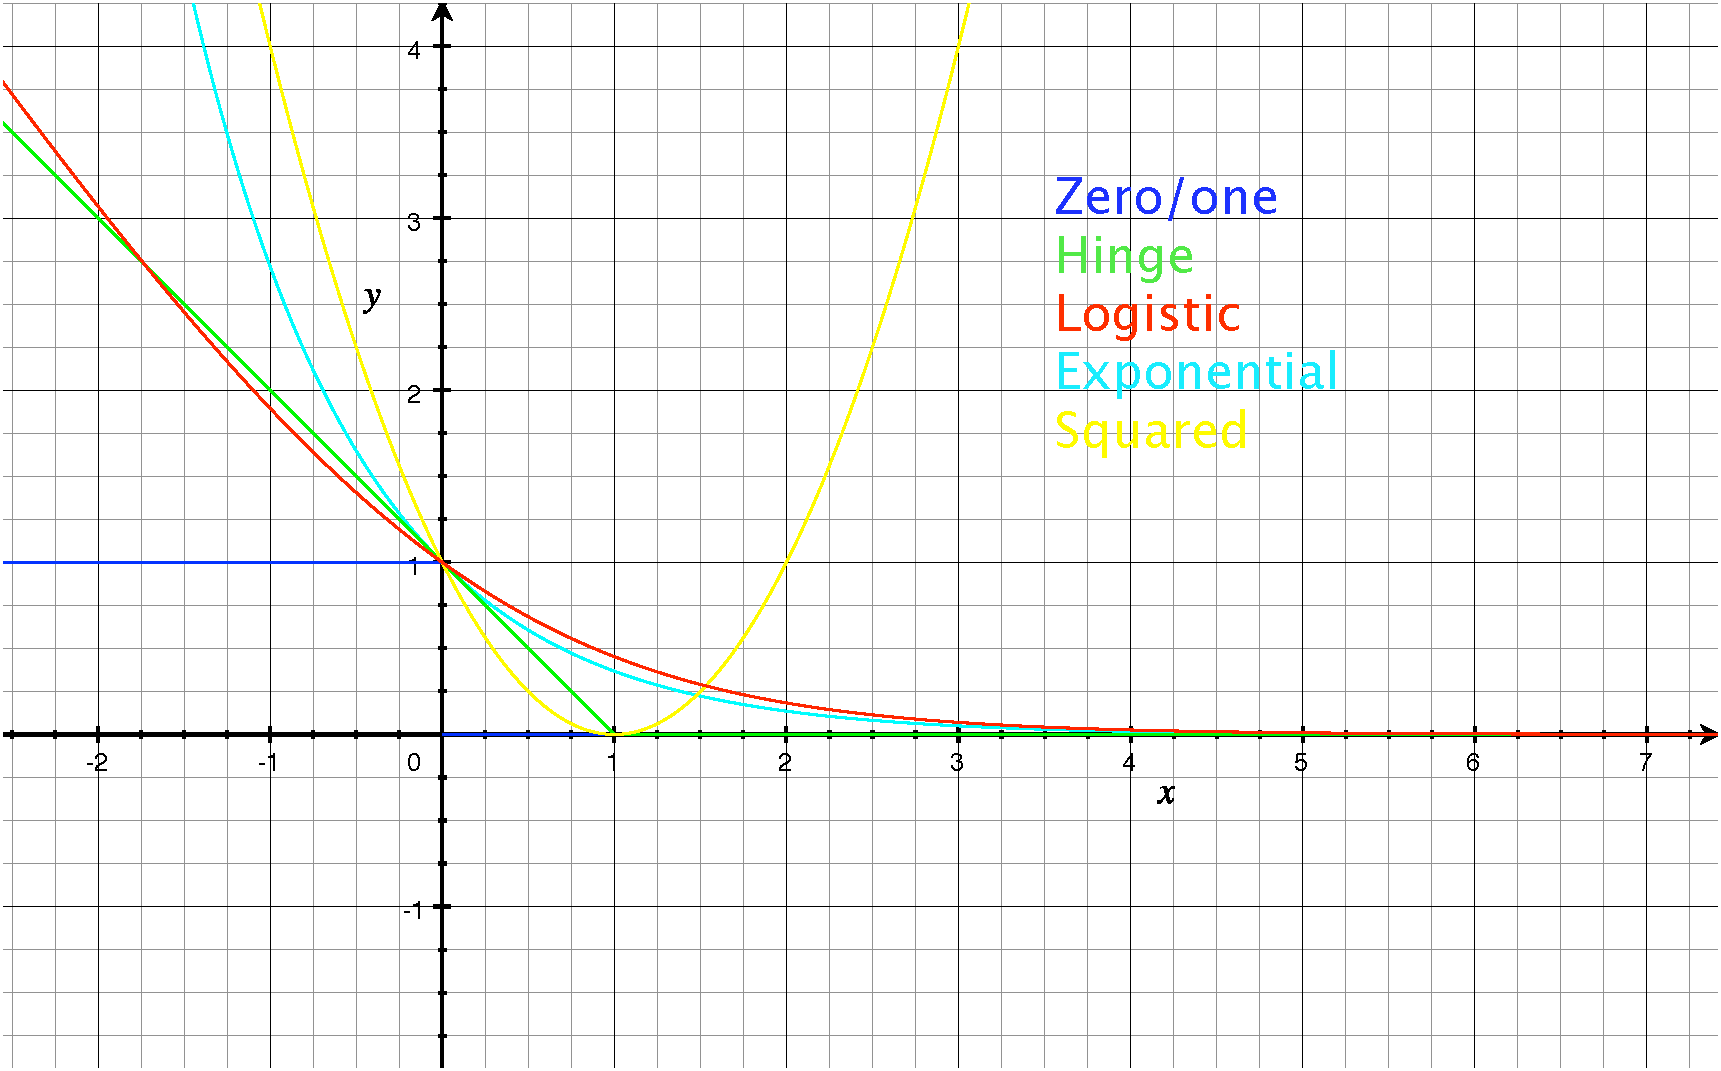
\includegraphics[width=0.65\textwidth]{loss}
\end{center}
\end{frame}

\begin{frame}
  \frametitle{Convex Surrogate Loss Functions}
\begin{itemize}
\item True label $y$ (which is just $\{-1,+1\}$) and
the predicted value $\hat y = \dotp{\vw}{\vx}+b$.
%
\begin{align}
\text{Zero/one:}    && \ell\xth{0/1}(y,\hat y) &= \Ind[y \hat y \leq 0] \\
\text{Hinge:}       && \ell\xth{hin}(y,\hat y) &= \max \{ 0, 1-y\hat y \}\\
\text{Logistic:}    && \ell\xth{log}(y,\hat y) &= \frac 1 {\log2} \log\left( 1 + \exp[-y\hat y]\right)\\
\text{Exponential:} && \ell\xth{exp}(y,\hat y) &= \exp[-y\hat y]\\
\text{Squared:}     && \ell\xth{sqr}(y,\hat y) &= (y-\hat y)^2=(1-y\hat y)^2
\end{align}
%
\end{itemize}
\end{frame}

\begin{frame}
  \frametitle{Convex Surrogate Loss Functions}
\begin{itemize}
\item
In the definition of logistic loss, the $\frac 1 {\log2}$ term ensures that $\ell\xth{log}(y,0) = 1$. 
\item  This
ensures, like all the other surrogate loss functions, that logistic
loss upper bounds the zero/one loss.  (In practice, people typically
omit this constant since it does not affect the optimization.)
\end{itemize}
\end{frame}

\begin{frame}
  \frametitle{Convex Surrogate Loss Functions}
\begin{itemize}
\item
Two big differences in these loss functions:
\begin{itemize}
\item How ``upset'' they get by erroneous predictions.  In the
case of hinge loss and logistic loss, the growth of the function as
$y\hat y$ goes negative is linear.  For squared loss and exponential
loss, it is super-linear.  This means that exponential loss would
rather get a few examples a little wrong than one example really
wrong. 
\item How they deal with very confident
correct predictions.  Once $y\hat y>1$, hinge loss does not care any
more, but logistic and exponential still think you can do better.  On
the other hand, squared loss thinks it's just as bad to predict $+3$
on a positive example as it is to predict $-1$ on a positive example.
\end{itemize}
\end{itemize}
\end{frame}

\section{Weight Regularization}

\begin{frame}
  \frametitle{Weight Regularization}
\begin{itemize}
\item
If you replace  zero/one loss with a
surrogate loss, you obtain the following objective:
%
\optimizeuc{loss:reg}{\vw,b}{%
  \sum_n \ell(y_n, \dotp{\vec w}{\vx_n}+b) + \la R(\vw,b)}
%
\item The question is: what should $R(\vw,b)$ look like?
\end{itemize}
\end{frame}

\begin{frame}
  \frametitle{Weight Regularization}
\begin{itemize}
\item
We would like to
ensure that $R$ is convex.  Otherwise  optimization becomes difficult.
\item The components of the weight vector (i.e., the $w_d$s) should be
small (close to zero).  This is a form of \concept{inductive bias}.
\item 
Why are small values of $w_d$ good?  Or, more precisely, why do small
values of $w_d$ correspond to \emph{simple functions}? 
\end{itemize}
\end{frame}

\begin{frame}
  \frametitle{Weight Regularization}
\begin{itemize}
\item  Suppose that
we have an example $\vx$ with label $+1$.  We might believe that other
examples, $\vx'$ that are nearby $\vx$ should also have label $+1$.
\item For example, if I obtain $\vx'$ by taking $\vx$ and changing the first
component by some small value $\ep$ and leaving the rest the same, you
might think that the classification would be the same.  
\item If you do
this, the difference between $\hat y$ and $\hat y'$ will be exactly
$\ep w_1$.  So if $w_1$ is reasonably small, this is unlikely to have
much of an effect on the classification decision. 
\item On the other hand,
if $w_1$ is large, this could have a large effect.
\end{itemize}
\end{frame}

\begin{frame}
  \frametitle{Weight Regularization}
\begin{itemize}
\item
 The derivative of
$\dotp{\vw}{\vx}+b$ with respect to $x_1$ is:
\begin{equation}
\frac {\partial \left[\dotp{\vw}{\vx}+b\right]} {\partial x_1}
= \frac {\partial \left[\sum_d w_d x_d+b\right]} {\partial x_1}
= w_1
\end{equation}
\item Interpreting the derivative as the rate of change, we can see that the
rate of change of the prediction function is proportional to the
individual weights. 
\item So if you want the function to change slowly, you
want to ensure that the weights stay small.
\end{itemize}
\end{frame}

\begin{frame}
  \frametitle{Weight Regularization}
\begin{itemize}
\item
One way to accomplish this is to simply use the norm of the weight
vector.  Namely $R\xth{norm}(\vw,b) = \norm{\vw} = \sqrt{\sum_d
  w_d^2}$.  
  \item This function is convex and smooth, which makes it easy to
minimize. 
\item  In practice, it's often easier to use the squared norm,
namely $R\xth{sqr}(\vw,b) = \norm{\vw}^2 = \sum_d w_d^2$ because it
removes the ugly square root term and remains convex. 
\item  An alternative
to using the sum of squared weights is to use the sum of absolute
weights: $R\xth{abs}(\vw,b) = \sum_d \ab{w_d}$.  Both of these norms
are convex.
\end{itemize}
\end{frame}

\begin{frame}
  \frametitle{Weight Regularization}
\begin{itemize}
\item
%\thinkaboutit{Why do we not regularize the bias term $b$?}
You could argue that
\emph{zero} weights are better.  
\item If a weight $w_d$ goes to zero, then
this means that feature $d$ is not used at all in the classification
decision.
\item   If there are a large number of irrelevant features, you
might want as many weights to go to zero as possible.  
\item Alternative regularizer: $R\xth{cnt}(\vw,b) = \sum_d \Ind[w_d \neq
0]$.
\end{itemize}
\end{frame}

\begin{frame}
  \frametitle{Weight Regularization}
\begin{itemize}
\item
%\thinkaboutit{Why might you not want to use $R\xth{cnt}$ as a regularizer?}
General concept of
\concept{$p$-norms}.  (Technically these are called $\ell_p$ (or ``ell
$p$'') norms, but this notation clashes with the use of $\ell$ for
``loss.'') 
\item Family of norms that all have the same general
flavor. 
\item We write $\norm{\vw}_p$ to denote the $p$-norm of $\vw$.
%
\begin{equation} \label{eq:loss:l}
  \norm{\vw}_p = \left( \sum_d \ab{w_d}^p \right)^{\frac 1 p}
\end{equation}
%
\item The $2$-norm exactly corresponds to the usual
Euclidean norm, and  the $1$-norm corresponds to the ``absolute''
regularizer described above.
\end{itemize}
\end{frame}

\begin{frame}
  \frametitle{Weight Regularization}
\begin{itemize}
\item
%\thinkaboutit{You can actually identify the $R\xth{cnt}$ regularizer
%  with a $p$-norm as well.  Which value of $p$ gives it to you?
%  (Hint: you may have to take a limit.)}
%\TODOFigure{loss:norms2d}{level sets of the same $p$-norms}
%When $p$-norms are used to regularize weight vectors, the interesting
%aspect is how they trade-off multiple features.  
We can plot their \concept{contour}
(or \concept{level-set}).
\item In two-dimensions by changing the value of $p$, you can interpolate between a
square (the so-called ``max norm''), down to a circle ($2$-norm),
diamond ($1$-norm) and pointy-star-shaped-thing ($p<1$ norm).
\item
%\thinkaboutit{The max norm corresponds to $\lim_{p \rightarrow
%    \infty}$.  Why is this called the max norm?}
In general, smaller values of $p$ ``prefer'' sparser vectors.  
\item You can
see this by noticing that the contours of small $p$-norms ``stretch''
out along the axes.
\item Small $p$-norms tend
to yield weight vectors with many zero entries (aka \concept{sparse}
weight vectors). 
\item For $p<1$ the norm becomes
non-convex.  
\item The $1$-norm is a
popular choice for sparsity-seeking applications.

\end{itemize}
\end{frame}
\section{Optimization with Gradient Descent}

\begin{frame}
  \frametitle{Optimization with Gradient Descent}
\begin{itemize}
\item
%\begin{mathreview}{Gradients}
%  ... be sure to do enough to do the closed for squared error
%\end{mathreview}
You're taking up a new hobby:
blindfolded mountain climbing.  
\item Someone blindfolds you and drops you
on the side of a mountain.  
\item Your goal is to get to the peak of the
mountain as quickly as possible. 
\item  All you can do is feel the mountain
where you are standing, and take steps. 
\item  How would you get to the top
of the mountain?  
\end{itemize}
\end{frame}

\begin{frame}
  \frametitle{Optimization with Gradient Descent}
\begin{itemize}
\item
Perhaps you would feel to find out what direction
feels the most ``upward'' and take a step in that direction. 
\item If you
do this repeatedly, you might hope to get the the top of the mountain.
(Actually, if your friend promises always to drop you on purely
concave mountains, you \emph{will} eventually get to the peak!)
\item
The idea of gradient-based methods of optimization is exactly the
same.
\end{itemize}
\end{frame}

\begin{frame}
  \frametitle{Optimization with Gradient Descent}
\begin{itemize}
\item
  Suppose you are trying to find the maximum of a function
$f(\vx)$.
\item  The optimizer maintains a current estimate of the parameter
of interest, $\vx$. 
\item At each step, it measures the \concept{gradient}
of the function it is trying to optimize. 
\item This measurement occurs
\emph{at} the current location, $\vx$.  Call the gradient $\vg$.
\item  It
then takes a step in the direction of the gradient, where the size of
the step is controlled by a parameter $\eta$ (eta).  
\item The complete step
is $\vx \leftarrow \vx + \eta \vg$.  This is the basic idea of
\concept{gradient ascent}.
\end{itemize}
\end{frame}

\begin{frame}
  \frametitle{Optimization with Gradient Descent}
\begin{itemize}
\item
The opposite of gradient ascent is \concept{gradient descent}.  
\item All of
our learning problems will be framed as \emph{minimization} problems
(trying to reach the bottom of a ditch, rather than the top of a
hill).  
\item Therefore, descent is the primary approach you will use.
\item One of the major conditions for gradient descent being able to find the
true, \concept{global minimum}, of its objective function is
convexity.  Without convexity, all is lost.
\end{itemize}
\end{frame}

\begin{frame}
  \frametitle{Optimization with Gradient Descent}
\newalgorithm{loss:gd}%
  {\FUN{GradientDescent}($\cF$, \VAR{K}, \VAR{$\eta_1$}, \dots)}
  {
\SETST{$\vz\zth$}{$\langle \CON0,\CON0, \dots, \CON0\rangle$}
  \COMMENT{initialize variable we are optimizing}
\FOR{\VAR{k} = \CON{1} \dots \VAR{K}}
\SETST{$\vg\kth$}{$\left. \grad_\vz \cF \right\vert_{\VARm{\vz\kpth}}$}
  \COMMENT{compute gradient at current location}
\SETST{$\vz\kth$}{$\VARm{\vz\kpth} - \VARm{\eta}\VARm{\kth} \VARm{\vg\kth}$}
  \COMMENT{take a step down the gradient}
\ENDFOR
\RETURN \VARm{$\vz\Kth$}
}
\end{frame}

\begin{frame}
  \frametitle{Optimization with Gradient Descent}
\begin{itemize}
\item
The function takes as arguments the
function $\cF$ to be minimized, the number of iterations $K$ to run
and a sequence of learning rates $\eta_1, \dots, \eta_K$. 
\item
The only real work you need to do to apply a gradient descent method
is be able to compute derivatives. 
\item Suppose that you
choose exponential loss as a loss function and the $2$-norm as a
regularizer. 
\end{itemize}
\end{frame}

\begin{frame}
  \frametitle{Optimization with Gradient Descent}
\begin{itemize}
\item  Then, the regularized objective function is:
%
\begin{equation}
\cL(\vw,b) =
\sum_n 
  \exp\big[-y_n (\dotp{\vec w}{\vx_n}+b)\big] +
 \frac \la 2 \norm{\vw}^2
\end{equation}
%
\item The only ``strange'' thing in this objective is that we have replaced
$\la$ with $\frac \la 2$.  The reason for this change is just to make
the gradients cleaner.  
\end{itemize}
\end{frame}

\begin{frame}
  \frametitle{Optimization with Gradient Descent}
\begin{itemize}
\item
We can first compute derivatives with respect
to $b$:
%
\begin{align}
\frac {\partial\cL} {\partial b}
&= \partialby{b}\sum_n \exp\big[-y_n (\dotp{\vec w}{\vx_n}+b)\big] + \partialby{b}\frac \la 2 \norm{\vw}^2\\
&= \sum_n \partialby{b} \exp\big[ -y_n (\dotp{\vec w}{\vx_n}+b)\big] + 0\\
&= \sum_n \left( \partialby{b} -y_n (\dotp{\vec w}{\vx_n}+b) \right) \exp\big[ -y_n (\dotp{\vec w}{\vx_n}+b)\big]\\
&= - \sum_n y_n \exp\big[ -y_n (\dotp{\vec w}{\vx_n}+b)\big]
\end{align}
%
\end{itemize}
\end{frame}

\begin{frame}
  \frametitle{Optimization with Gradient Descent}
\begin{itemize}
\item
The optimization will operate by updating $b
\leftarrow b - \eta \partialof{\cL}{b}$.  
\item Consider positive examples:
examples with $y_n=+1$. 
\item  We would hope for these examples that the
current prediction, $\dotp{\vw}{\vx_n}+b$, is as large as possible.
\item 
As this value tends toward $\infty$, the term in the $\exp[]$ goes to
zero.  Thus, such points will not contribute to the step.  
\item However, if
the current prediction is small, then the $\exp[]$ term will be
positive and non-zero.  
\item This means that the bias term $b$ will be
\emph{increased}, which is exactly what you would want.
\item  Moreover,
once all points are very well classified, the derivative goes to zero.
\end{itemize}
\end{frame}

\begin{frame}
  \frametitle{Optimization with Gradient Descent}
\begin{itemize}
\item
%\thinkaboutit{This considered the case of positive examples.  What
%  happens with negative examples?}
Gradient with
respect to $\vw$.
%
\begin{align}
\grad_\vw \cL
&= \grad_\vw \sum_n \exp\big[-y_n (\dotp{\vec w}{\vx_n}+b)\big] 
 + \grad_\vw\frac \la 2 \norm{\vw}^2 \\
&= \sum_n \left( \grad_\vw -y_n (\dotp{\vec w}{\vx_n}+b) \right) \exp\big[-y_n (\dotp{\vec w}{\vx_n}+b)\big] 
 + \la \vw \\
&= -\sum_n y_n \vx_n \exp\big[-y_n (\dotp{\vec w}{\vx_n}+b)\big] 
 + \la \vw
\end{align}
%
\end{itemize}
\end{frame}

\begin{frame}
  \frametitle{Optimization with Gradient Descent}
\begin{itemize}
\item
Update of the form
$\vw \leftarrow \vw - \eta \grad_\vw \cL$.  
\item For well classified points
(ones that tend toward $y_n \infty$), the gradient is near zero.
\item For poorly classified points, the gradient points in the direction
$-y_n\vx_n$, so the update is of the form $\vw \leftarrow \vw + c
y_n\vx_n$, where $c$ is some constant.  
\item This is just like the
perceptron update! 
\item  Note that $c$ is large for very poorly classified
points and small for relatively well classified points.
\end{itemize}
\end{frame}

\begin{frame}
  \frametitle{Optimization with Gradient Descent}
\begin{itemize}
\item
By looking at the part of the gradient related to the regularizer, the
update says: $\vw \leftarrow \vw - \la \vw = (1-\la) \vw$.  
\item This has
the effect of \emph{shrinking} the weights toward zero.  This is
exactly what we expect the regulaizer to be doing!
\end{itemize}
\end{frame}

\begin{frame}
  \frametitle{Optimization with Gradient Descent}
\begin{itemize}
\item
The success of gradient descent hinges on appropriate choices for the
step size.
\item With a poorly chosen step size:
\Figure{loss:step}{good and bad step sizes}{0.3}
\item If the step size is
too big, you can accidentally step over the optimum and end up
oscillating.
\item   If the step size is too small, it will take way too long
to get to the optimum.  
\end{itemize}
\end{frame}

\begin{frame}
  \frametitle{Optimization with Gradient Descent}
\begin{itemize}
\item For a well-chosen step size, you can show that
gradient descent will approach the optimal value at a fast
\emph{rate}.
\item   The notion of convergence here is that the
\emph{objective value} converges to the true minimum.
\begin{theorem}[Gradient Descent Convergence] \label{thm:loss:gd}
  Under suitable conditions%\sidenote{Specifically the function to be
%    optimized needs to be \concept{strongly convex}.  This is true for
%    all our problems, provided $\la>0$.  For $\la=0$ the rate could be
%    as bad as $\cO(1/\sqrt{k})$.}
    , for an appropriately chosen
  constant step size (i.e., $\eta_1 = \eta_2, \dots = \eta$), the
  \concept{convergence rate} of gradient descent is $\cO(1/k)$.  More
  specifically, letting $\vz^*$ be the global minimum of $\cF$, we
  have: $\cF(\vz\kth) - \cF(\vz^*) \leq \frac {2
    \norm{\vz\zth-\vz^*}^2} {\eta k}$.
\end{theorem}
\end{itemize}
\end{frame}

%\begin{frame}
%  \frametitle{Optimization with Gradient Descent}
%\begin{itemize}
%\item
%%\thinkaboutit{A naive reading of this theorem seems to say that you
%%  should choose huge values of $\eta$.  It should be obvious that this
%%  cannot be right.  What is missing?}
%The proof of this theorem is a bit complicated because it makes heavy
%use of  linear algebra.  
%\end{itemize}
%\end{frame}




\begin{comment}
Fortunately, we can prove a simpler version of this theorem for
one-dimensional functions.  We do this just to give a sense of how
convergence proofs go.  In the single dimensional case, we will call
the algorithm ``derivative descent.''  To set up some notation, let
$f(z)$ be the function to be minimized by derivative descent.  Let
$z_0$ be the initial value and $z^*$ be the optimum.  Let $f'(z)$ be
the first derivative of $f$ and let $f''$ be the second derivative.
Let $L$ be large enough that $f''(z) < L$ for all $z$.

\begin{theorem}[Derivative Descent Convergence] \label{thm:loss:dd}
  For constant $\eta = 1/L$, derivative descent will converge at a
  rate of $f(z\kth) - f(z^*) \leq \frac {2 (z\zth-z^*)^2} {\eta(k+1)}$.
\end{theorem}

\begin{myproof}{\ref{thm:loss:dd}}
  We use Taylor's theorem to expand $f(z)$:
  \begin{align}
    f(z)
      &= f(a)
       + f'(a) (z-a)
       + \frac 1 2 f''(a) (z-a)^2
       + \dots \\
      &\leq f(a)
       + f'(a) (z-a)
       + \frac 1 2 f''(a) (z-a)^2
  \end{align}
  The ``\dots'' is guaranteed to be non-negative because $f$ is
  convex.  
\end{myproof}
\end{comment}
\begin{frame}
  \frametitle{Optimization with Gradient Descent}
\begin{itemize}
\item
This convergence result suggests a simple approach to deciding when to
stop optimizing: wait until the objective function stops changing by
much.  
\item An alternative is to wait until the \emph{parameters} stop
changing by much. 
\item A final example is to do what you did for
perceptron: early stopping.  
\item Every iteration, you can check the
performance of the current model on some held-out data, and stop
optimizing when performance plateaus.
\end{itemize}
\end{frame}

\section{From Gradients to Subgradients}
\begin{frame}
  \frametitle{From Gradients to Subgradients}
\begin{itemize}
\item The $1$-norm is not differentiable around
$w_d=0$, and the hinge loss is not differentiable around $y\hat y=1$.
\item 
The solution to this is to use \concept{subgradient} optimization.
\item One way to think about subgradients is just to not think about it: you
essentially need to just ignore the fact that  your
function isn't differentiable, and just try to apply gradient descent
anyway.
\item 
Consider the hinge function $f(z) =
\max\{0,1-z\}$. 
\item  This
function is differentiable for $z>1$ and differentiable for $z<1$, but
not differentiable at $z=1$. 
\end{itemize}
\end{frame}

\begin{frame}
  \frametitle{From Gradients to Subgradients}
\begin{itemize}
\item 
 You can derive this using
differentiation by parts:
%
\begin{align}
  \partialby{z} f(z)
  &= \partialby{z} \brack{ 0 & \txtif z > 1 \\ 1-z & \txtif z < 1} \\
  &= \brack{ \partialby{z} 0 & \txtif z > 1 \\ \partialby{z} (1-z) & \txtif z < 1}\\
  &= \brack{ 0 & \txtif z > 1 \\ -1 & \txtif z < 1}
\end{align}
%
\end{itemize}
\Figure{loss:sub}{hinge loss with sub}{0.3}
\end{frame}

\begin{frame}
  \frametitle{From Gradients to Subgradients}
\begin{itemize}
\item 
  At the non-differentiable point, $z=1$, we
can use a \concept{subderivative}: a generalization of derivatives to
non-differentiable functions.
\item You can think of the
derivative of $f$ at $z$ as the tangent line.
\item It is the line
that touches $f$ at $z$ that is always below $f$ (for convex
functions). 
\item The subderivative, denoted $\subgrad f$, is the
\emph{set} of all such lines.
\item  At differentiable positions, this set
consists just of the actual derivative.
\item  At non-differentiable
positions, this contains all slopes that define lines that always lie
under the function and make contact at the operating point. 
\end{itemize}
\end{frame}

\begin{frame}
  \frametitle{From Gradients to Subgradients}
\begin{itemize}
\item 
In the
particular case of hinge loss, any value between $0$ and $-1$ is a
valid subderivative at $z=0$.
\item The subderivative is always a
closed set of the form $[a,b]$, where $a$ and $b$ can be derived by
looking at limits from the left and right.
\end{itemize}
\end{frame}

\begin{frame}
  \frametitle{From Gradients to Subgradients}
\begin{itemize}
\item 
This gives you a way of computing derivative-like things for
non-differentiable functions. 
\item Take hinge loss as an example.  For a
given example $n$, the subgradient of hinge loss can be computed as:
%
\begin{align}
&\subgrad_\vw \max \{ 0, 1 - y_n ( \dotp{\vw}{\vx_n}+b ) \} \\
&= \subgrad_\vw \brack{ 0 & \txtif y_n ( \dotp{\vw}{\vx_n}+b ) > 1 \\
                        1 - y_n ( \dotp{\vw}{\vx_n}+b )  & \text{otherwise}}\\
&= \brack{ \subgrad_\vw 0 & \txtif y_n ( \dotp{\vw}{\vx_n}+b ) > 1 \\
           \subgrad_\vw 1 - y_n ( \dotp{\vw}{\vx_n}+b )  & \text{otherwise}}\\
&= \brack{ \vec 0 & \txtif y_n ( \dotp{\vw}{\vx_n}+b ) > 1 \\
           - y_n \vx_n  & \text{otherwise}}
\end{align}
\end{itemize}
\end{frame}

\begin{frame}
  \frametitle{\concept{Subgradient descent} for regularized hinge loss (with a
$2$-norm regularizer)}
\newalgorithm%
  {loss:gdhinge}%
  {\FUN{HingeRegularizedGD}(\VAR{$\mat D$}, \VAR{$\la$}, \VAR{MaxIter})}
  {
\SETST{$\vw$}{$\langle \CON{0}, \CON{0}, \dots \CON{0} \rangle$
  \quad,\quad
  \VAR{$b$} $\leftarrow$ \CON{0}}
  \COMMENT{initialize weights and bias}
\FOR{\VAR{iter} = \CON{1} \dots \VAR{MaxIter}}
\SETST{$\vg$}{$\langle \CON{0}, \CON{0}, \dots \CON{0} \rangle$
  \quad,\quad
  \VAR{$g$} $\leftarrow$ \CON{0}}
  \COMMENT{initialize gradient of weights and bias}
\FORALL{(\VAR{$\vx$},\VAR{$y$}) $\in$ \VAR{$\mat D$}}
\IF{\VAR{$y$}$\left( \dotp{\VARm{\vw}}{\VARm{\vx}} + \VARm{b} \right) \leq \CON{1}$}
\SETST{$\vg$}{\VAR{$\vg$} + \VAR{$y$} \VAR{$\vx$}}
  \COMMENT{update weight gradient}
\SETST{$g$}{\VAR{$g$} + \VAR{$y$}}
  \COMMENT{update bias derivative}
\ENDIF
\ENDFOR
\SETST{$\vg$}{$\VARm{\vg} - \VARm{\la} \VARm{\vw}$}
  \COMMENT{add in regularization term}
\SETST{$\vw$}{$\VARm{\vw} + \VARm{\eta} \VARm{\vg}$}
  \COMMENT{update weights}
\SETST{$b$}{$\VARm{b} + \VARm{\eta} \VARm{g}$}
  \COMMENT{update bias}
\ENDFOR
\RETURN \VAR{$\vw$}, \VAR{$b$}
}
\end{frame}
\section{Closed-form Optimization for Squared Loss}
\label{sec:loss:reg}

\begin{frame}
  \frametitle{Closed-form Optimization for Squared Loss}
\begin{itemize}
\item 
%\begin{mathreview}{Matrix multiplication and inversion}
%  \dots
%\end{mathreview}
Although gradient descent is a good, generic optimization algorithm,
there are cases when you can do better. 
\item An example is the case of a
$2$-norm regularizer and squared error loss function.
\item  For this, you
can actually obtain a \emph{closed form} solution for the optimal
weights. 
\item To obtain this, you need to rewrite the
optimization problem in terms of matrix operations. 
\item  For simplicity,
we will only consider the \emph{unbiased} version
\item
This is precisely the \concept{linear regression}
setting.
\end{itemize}
\end{frame}

\begin{frame}
  \frametitle{Closed-form Optimization for Squared Loss}
\begin{itemize}
\item 
You can think of the training data as a large matrix $\mat X$ of size
$N \times D$, where $X_{n,d}$ is the value of the $d$th feature on the
$n$th example. 
\item  You can think of the labels as a column (``tall'')
vector $\vec Y$ of dimension $N$.
\item  Finally, you can think of the
weights as a column vector $\vec w$ of size $D$. 
\item Thus, the
matrix-vector product $\vec a = \mat X \vec w$ has dimension $N$.
\end{itemize}
\end{frame}

\begin{frame}
  \frametitle{Closed-form Optimization for Squared Loss}
\begin{itemize}
\item 
  In
particular:
%
\begin{equation}
a_n
= \left[ \mat X \vec w \right]_n 
= \sum_d \mat X_{n,d} w_d
\end{equation}
%
\item  $\vec a$ is actually the predictions
of the model.
\item  Instead of calling this $\vec a$, we will call it
$\hat{\vec Y}$. 
\item The squared error says that we should minimize $\frac 1
2 \sum_n (\hat Y_n - Y_n)^2$, which can be written in vector form as a
minimization of $\frac 1 2 \norm{\hat{\vec Y} - \vec Y}^2$.
\end{itemize}
\end{frame}

\begin{frame}
  \frametitle{Closed-form Optimization for Squared Loss}
\begin{itemize}
\item 
%\thinkaboutit{Verify that the squared error can actually be written as
%  this vector norm.}
This can be expanded visually as:
%
\begin{equation}
\underbrace{
\textcolor{darkblue}{
\left[
\begin{array}{cccc}
  x_{1,1} & x_{1,2} & \dots & x_{1,D} \\
  x_{2,1} & x_{2,2} & \dots & x_{2,D} \\
  \vdots & \vdots & \ddots & \vdots \\
  x_{N,1} & x_{N,2} & \dots & x_{N,D}
\end{array}
\right]
}}_{\textcolor{darkblue}{\mat X}}
\underbrace{
\textcolor{darkergreen}{
\left[
\begin{array}{c}
  w_{1} \\
  w_{2} \\ 
  \vdots \\
  w_{D}
\end{array}
\right]
}}_{\textcolor{darkergreen}{\vec w}}
=
\underbrace{
\left[
\begin{array}{c}
  \sum_d \textcolor{darkblue}{x_{1,d}} \textcolor{darkergreen}{w_d} \\
  \sum_d \textcolor{darkblue}{x_{2,d}} \textcolor{darkergreen}{w_d} \\
  \vdots \\
  \sum_d \textcolor{darkblue}{x_{N,d}} \textcolor{darkergreen}{w_d}
\end{array}
\right]
}_{\vec{\hat Y}}
%\approx
%\underbrace{
%\textcolor{darkred}{
%\left[
%\begin{array}{c}
%  y_{1} \\
%  y_{2} \\ 
%  \vdots \\
%  y_{N}
%\end{array}
%\right]
%}}_{\textcolor{darkred}{\vec{\hat Y}}}
\end{equation}
\end{itemize}
\end{frame}

\begin{frame}
  \frametitle{Closed-form Optimization for Squared Loss}
\begin{itemize}
\item 
%
So, compactly, our optimization problem can be written as:
%
\optimizeuc{loss:squarederror}{\vw}{%
  \cL(\vw) =
  \frac 1 2 \norm{\mat X \vw - \vec Y}^2 + \frac \la 2 \norm{\vw}^2}
%
\item If you recall from calculus, you can minimize a function by setting
its derivative to zero.  We start with the weights $\vw$ and take
gradients:
%
\begin{align}
\grad_\vw \cL(\vw)
&= \mat X \T \left( \mat X \vw - \vec Y \right) + \la \vw \\
&= \mat X \T \mat X \vw - \mat X \T \vec Y + \la \vw \\
&= \left( \mat X \T \mat X + \la \eye \right) \vw - \mat X \T \vec Y
\end{align}
%
\end{itemize}
\end{frame}

\begin{frame}
  \frametitle{Closed-form Optimization for Squared Loss}
\begin{itemize}
\item We can equate this to zero and solve, yielding:
%
\begin{align}
     & \textcolor{darkblue}{\left( \mat X \T \mat X + \la \eye \right)} \textcolor{darkred}{\vw} - \textcolor{darkergreen}{\mat X \T \vec Y} = 0\\
\myiff~~ & \textcolor{darkblue}{\left( \mat X \T \mat X + \la \eye_D \right)} \textcolor{darkred}{\vw} = \textcolor{darkergreen}{\mat X \T \vec Y} \\
\myiff~~ & \textcolor{darkred}{\vw} = \textcolor{darkblue}{\left( \mat X \T \mat X + \la \eye_D \right)}\inv \textcolor{darkergreen}{\mat X \T \vec Y}
\end{align}
%
\end{itemize}
\end{frame}

\begin{frame}
  \frametitle{Closed-form Optimization for Squared Loss}
\begin{itemize}
\item Thus, the \emph{optimal} solution of the weights can be computed by a
few matrix multiplications and a matrix inversion.
%
\item As a sanity check, you can make sure that the dimensions match.
\item  The
matrix $\mat X\T\mat X$ has dimension $D\times D$, and therefore so
does the inverse term.  
\item The inverse is $D\times D$ and $\mat X\T$ is
$D\times N$, so that product is $D\times N$.  
\item Multiplying through by
the $N\times 1$ vector $\vec Y$ yields a $D \times 1$ vector, which is
precisely what we want for the weights.
\end{itemize}
\end{frame}

\begin{frame}
  \frametitle{Closed-form Optimization for Squared Loss}
\begin{itemize}
%\thinkaboutit{For those who are keen on linear algebra, you might be
%  worried that the matrix you must invert might not be invertible.  Is
%  this actually a problem?}
\item This gives an \emph{exact solution}, modulo numerical
innacuracies with computing matrix inverses. 
\item In contrast, gradient
descent will give you progressively better solutions and will
``eventually'' converge to the optimum at a rate of $1/k$.  
\item This means
that if you want an answer that's within an accuracy of $\ep =
10^{-4}$, you will need something on the order of one thousand steps.
\end{itemize}
\end{frame}

\begin{frame}
  \frametitle{Closed-form Optimization for Squared Loss}
\begin{itemize}
\item 
The question is whether getting this exact solution is always more
efficient.
\item  To run gradient descent for one step will take $\cO(ND)$
time, with a relatively small constant.
\item  You will have to run $K$
iterations, yielding an overall runtime of $\cO(KND)$.  
\item The closed form solution requires constructing $\mat X\T\mat X$,
which takes $\cO(D^2 N)$ time. 
\item The inversion take $\cO(D^3)$ time
using standard matrix inversion routines.  The final multiplications
take $\cO(ND)$ time.  Thus, the overall runtime is on the order
$\cO(D^3 + D^2 N)$.  
\item In most standard cases (though this is becoming
less true over time), $N > D$, so this is dominated by $\cO(D^2 N)$.
\end{itemize}
\end{frame}

\begin{frame}
  \frametitle{Closed-form Optimization for Squared Loss}
\begin{itemize}
\item 
The overall question is whether you will need to run more than
$D$-many iterations of gradient descent.  
\item If so, then the matrix
inversion will be (roughly) faster.
\item For low- and medium-dimensional problems (say,
$D \leq 100$), it is probably faster to do the closed form solution
via matrix inversion. 
\item  For high dimensional problems ($D \geq
10,000$), it is probably faster to do gradient descent.  For things in
the middle, it's hard to say for sure.
\end{itemize}
\end{frame}

\section{Support Vector Machines} \label{sec:loss:svm}

\begin{frame}
  \frametitle{Support Vector Machines}
\begin{itemize}
\item 
% TODO: bias/variance trade-off???
Convex
surrogate loss functions are all derived from different underlying principles,
which essentially correspond to different inductive biases.  
\item
Original goal of linear
classifiers: to find a hyperplane that separates the positive training
examples from the negative ones.
\Figure{loss:geom}{picture of data points with three hyperplanes,
  RGB with G the best}{0.3}
\item Three potential hyperplanes: red, green and blue.  Which
one do you like best?
\end{itemize}
\end{frame}


\begin{frame}
  \frametitle{Support Vector Machines}
\begin{itemize}
\item 
Most likely you chose the green hyperplane because it was furthest away from the closest training points. 
\item In
other words, it had a large \concept{margin}. 
\item  The desire for
hyperplanes with large margins is a perfect example of an inductive
bias. 
\item  The data does not tell us which of the three hyperplanes is
best: we have to choose one using some other source of information.
\end{itemize}
\end{frame}


\begin{frame}
  \frametitle{Support Vector Machines}
\begin{itemize}
\item 
 \concept{Support
  vector machine} (SVM): a way of setting up an
optimization problem that attempts to find a separating hyperplane
with as large a margin as possible. 
\item  It is written as a
\concept{constrained optimization problem}:
%
\optimize{loss:svmhard}{\vw,b}{\frac 1 {\ga(\vw,b)}}{%
  y_n \left( \dotp{\vw}{\vx_n} + b \right) \geq 1& (\forall n)
%\nonumber &
%  \norm{\vw} \leq 1
}
%
\end{itemize}
\end{frame}

\begin{frame}
  \frametitle{Support Vector Machines}
\begin{itemize}
\item 
In this optimization, you are trying to find parameters that maximize
the margin, denoted $\ga$, (i.e., minimize the reciprocal of the
margin) subject to the constraint that \emph{all} training examples
are correctly classified.
\end{itemize}
\end{frame}


\begin{comment}
There are two aspects of this optimization problem that are not
immediately obvious.  The first is the constraint that the norm of the
weight vector is at most $1$.  This constraint is necessary in order
to avoid degenerate solutions.  In particular, suppose you solved the
optimization problem \emph{with} this constraint in place.  You found
some optimal solution $\vw^*,b^*$.  Now, consider what happens if you
were to remove the norm constraint.  You could then look at
$2\vw^*,2b$.  The constraints would still be satisfied, but you would
have \emph{doubled} the size of the margin!  You could do this again,
eventually getting an infinitely large margin with $\infty\vw^*,\infty
b$ as parameters.  The constraint on the norm of $\vw$ is to ensure
that this doesn't happen.

%\thinkaboutit{You can also think about the constraint on $\vw$ in
%  terms of the fact that it's not $\vw$ we care about, but rather the
%  hyperplane it defines.  Why does this suggest that constraining the
%  norm of $\vw$ is reasonable?}
\end{comment}

\begin{frame}
  \frametitle{Support Vector Machines}
\begin{itemize}
\item 
The ``odd'' thing about this optimization problem is that we require
the classification of each point to be greater than \emph{one} rather
than simply greater than \emph{zero}.  
\item However, the problem doesn't
fundamentally change if you replace the ``1'' with any other positive
constant
\Figure{loss:margin}{hyperplane with margins on sides}{0.28}
\item The constant one can be interpreted
visually as ensuring that there is a non-trivial margin between the
positive points and negative points.
\end{itemize}
\end{frame}
\begin{frame}
  \frametitle{Support Vector Machines}
\begin{itemize}
\item 
The difficulty with the optimization problem is what happens with data that is not
linearly separable.  
\item There \emph{is no} set of
parameters $\vw,b$ that can simultaneously satisfy all the
constraints.
\item   In optimization terms, you would say that the
\concept{feasible region} is \emph{empty}.  (The feasible region is
simply the set of all parameters that satify the constraints.)  
\item For
this reason, this is refered to as the \concept{hard-margin SVM},
because enforcing the margin is a hard constraint. 
\end{itemize}
\end{frame}
\begin{frame}
  \frametitle{Support Vector Machines}
\begin{itemize}
\item 
The key idea is the use of \concept{slack parameters}.  
\item Suppose we find a set of
parameters $\vw,b$ that do a really good job on $9999$ data points.
\item The points are perfectly classifed and you achieve a large margin.
\item But there's one pesky data point left that cannot be put on the proper
side of the margin: perhaps it is noisy. 
\Figure{loss:slack}{one bad point with slack}{0.3}
\end{itemize}
\end{frame}
\begin{frame}
  \frametitle{Support Vector Machines}
\begin{itemize}
\item   You want to be able to pretend that you
can ``move'' that point across the hyperplane on to the proper side.
\item 
You will have to pay a little bit to do so, but as long as you aren't
moving a \emph{lot} of points around, it should be a good idea to do
this.  
\item The amount that you move the point is denoted
$\xi$ (xi).
\end{itemize}
\end{frame}
\begin{frame}
  \frametitle{Support Vector Machines}
\begin{itemize}
\item 
By introducing one slack parameter for each training example, and
penalizing yourself for having to use slack, you can create an
objective function like the following, \concept{soft-margin SVM}:
%
\optimize{loss:svm}{\vw,b,\vec\xi}{%
  \underbrace{\frac 1 {\ga(\vw,b)}}_{\text{large margin}}
+ \underbrace{C \sum_n \xi_n}_{\text{small slack}}
}{%
  y_n \left( \dotp{\vw}{\vx_n} + b \right) \geq 1 - \xi_n & (\forall n) \\
\nonumber &
  \xi_n \geq 0 & (\forall n)
%\nonumber &
%  \norm{\vw} \leq 1
}
%
\item The goal of this objective function is to ensure that all points are
correctly classified (the first constraint).
\item  But if a point $n$
cannot be correctly classified, then you can set the slack $\xi_n$ to
something greater than zero to ``move'' it in the correct direction.
\end{itemize}
\end{frame}
\begin{frame}
  \frametitle{Support Vector Machines}
\begin{itemize}
\item 
For all non-zero slacks, you have to pay in the objective
function proportional to the amount of slack. 
\item  The hyperparameter
$C>0$ controls overfitting versus underfitting.  
\item The second constraint
simply says that you must not have negative slack.
\end{itemize}
\end{frame}
\begin{frame}
  \frametitle{Support Vector Machines}
\begin{itemize} 
%\thinkaboutit{What values of $C$ will lead to overfitting?  What
%  values will lead to underfitting?}
\item 
One major advantage of the soft-margin SVM over the original
hard-margin SVM is that the feasible region is \emph{never empty}.
\item That is, there is always going to be some solution, regardless of
whether your training data is linearly separable or not.
%\thinkaboutit{Suppose I give you a data set.  Without even looking at
%  the data, construct for me a feasible solution to the soft-margin
%  SVM.  What is the value of the objective for this solution?}
\item 
It's one thing to write down an optimization problem.  It's another
thing to try to solve it.
\item   There are a very large number of ways to
optimize SVMs, essentially because they are such a popular learning
model.
\end{itemize}
\end{frame}
\begin{frame}
  \frametitle{Support Vector Machines}
\begin{itemize}
\item 
To make progress, you need to be able to measure the size of the
margin. 
\item Suppose someone gives you parameters $\vw,b$ that optimize
the hard-margin SVM.  
\item 
The
first observation is that the hyperplane will lie \emph{exactly}
halfway between the nearest positive point and nearest negative point.
\item If not, the margin could be made bigger by simply sliding it one way
or the other by adjusting the bias $b$.
\end{itemize}
\end{frame}
\begin{frame}
  \frametitle{Support Vector Machines}
\begin{itemize}
\item The distance from any point $\vx$ to the decision surface is $\frac{|\dotp{\vw}{\vx}+b|}{\norm{\vw}}$.
\item 
There is some positive example that that lies
exactly $1$ unit from the hyperplane.  Call it $\vx^+$, so that
$\dotp{\vw}{\vx^+}+b = 1$.
\item If not, we can rescale $\vw$ and $b$: $\vw\rightarrow \kappa\vw$, $b\rightarrow \kappa b$
so that $\dotp{\vw}{\vx^+}+b = 1$ without changing the distance.
\item  Similarly, there is some negative example,
$\vx^-$, that lies exactly on the other side of the margin: for which
$\dotp{\vw}{\vx^-}+b = -1$. 
\end{itemize}
\end{frame}
%\begin{frame}
%  \frametitle{Support Vector Machines}
%\Figure{loss:marginsize}{copy of figure from p5 of cs544 svm tutorial}{0.28}
%\begin{itemize}
%\item We can measure the size of the margin by
%looking at the difference between the lengths of projections of
%$\vx^+$ and $\vx^-$ onto $\vw$.  
%\end{itemize}
%\end{frame}
\begin{frame}
  \frametitle{Support Vector Machines}
\begin{itemize}
\item We can measure the size of the margin by
looking at the difference between the lengths of projections of
$\vx^+$ and $\vx^-$ onto $\vw$.  
\item 
We can measure the distances as:
%
\begin{align}
d^+ &= \frac 1 {\norm{\vw}} (|\dotp{\vw}{\vx^+} + b|) \\
d^- &=  \frac 1 {\norm{\vw}}(|\dotp{\vw}{\vx^-} + b|) 
\end{align}
%
\end{itemize}
\end{frame}
\begin{frame}
  \frametitle{Support Vector Machines}
\begin{itemize}
\item We can then compute the margin by algebra:
%
\begin{align}
\ga
&= \frac 1 2 \left[ \textcolor{darkblue}{d^+} 
                  +\textcolor{darkred}{d^-} \right] \\
&= \frac 1 2
   \left[
   \textcolor{darkblue}{\frac 1 {\norm{\vw}} (|\dotp{\vw}{\vx^+} + b|) }
 + \textcolor{darkred}{\frac 1 {\norm{\vw}} (|\dotp{\vw}{\vx^-} +b|) }
   \right]
%\\
%&= \frac 1 2 \left[
%   \textcolor{darkblue}{\frac 1 {\norm{\vw}} \dotp{\vw}{\vx^+}}
% - \textcolor{darkred}{\frac 1 {\norm{\vw}} \dotp{\vw}{\vx^-}}
% \right]
\\
&= \frac 1 2 \left[
   \textcolor{darkblue}{\frac 1 {\norm{\vw}} (+1) }
 +\textcolor{darkred}{\frac 1 {\norm{\vw}} (+1) }
 \right]
\\
&= \frac 1 {\norm{\vw}}
\end{align}
%
\end{itemize}
\end{frame}
\begin{frame}
  \frametitle{Support Vector Machines}
\begin{itemize}
\item 
This is a remarkable conclusion: the size of the margin is inversely
proportional to the norm of the weight vector.
\item   Thus, {\bf maximizing
  the margin is equivalent to minimizing $\norm{\vw}$!}  
  \item This serves
as an additional justification of the $2$-norm regularizer: having
small weights means having large margins!
\end{itemize}
\end{frame}
\begin{frame}
  \frametitle{Support Vector Machines}
\begin{itemize}
\item 
However, our goal wasn't to justify the regularizer: it was to
understand hinge loss.
\item   Let us go back to the soft-margin SVM and
plug in our new knowledge about margins:
%
\optimize{loss:svms}{\vw,b,\vec\xi}{%
  \underbrace{\frac 1 2 \norm{\vw}^2}_{\text{large margin}}
+ \underbrace{C \sum_n \xi_n}_{\text{small slack}}
}{%
  y_n \left( \dotp{\vw}{\vx_n} + b \right) \geq 1 - \xi_n & (\forall n) \\
\nonumber &
  \xi_n \geq 0 & (\forall n)
}
%
\item Here the margin is squared but the square is a monotonically increasing function
of its argument
\end{itemize}
\end{frame}
\begin{frame}
  \frametitle{Support Vector Machines}
\begin{itemize}
\item 
Now, let's play a thought experiment.  Suppose someone handed you a
solution to this optimization problem that consisted of weights
($\vw$) and a bias ($b$), but they forgot to give you the slacks.
\item 
Could you recover the slacks from the information you have?
\item
In fact, the answer is yes!  For simplicity, let's consider positive
examples. 
\item  Suppose that you look at some positive example $\vx_n$.
You need to figure out what the slack, $\xi_n$, would have been.
\item 
There are two cases.  Either $\dotp{\vw}{\vx_n}+b$ is at least $1$ or
it is not.
\item   If it's large enough, then you want to set $\xi_n = 0$.
\item
Why?  It cannot be less than zero by the second constraint.  Moreover,
if you set it greater than zero, you will ``pay'' unnecessarily in the
objective. 
\item  So in this case, $\xi_n=0$. 
\end{itemize}
\end{frame}
\begin{frame}
  \frametitle{Support Vector Machines}
\begin{itemize}
\item 
 Next, suppose that
$\dotp{\vw}{\vx_n}+b = 0.2$, so it is not big enough.  
\item In order to
satisfy the first constraint, you'll need to set $\xi_n \geq 0.8$.
\item But because of the objective, you'll not want to set it any larger
than necessary, so you'll set $\xi_n = 0.8$ exactly.
\end{itemize}
\end{frame}
\begin{frame}
  \frametitle{Support Vector Machines}
\begin{itemize}
\item 
Following this argument through for both positive and negative points,
if someone gives you solutions for $\vw,b$, you can automatically
compute the optimal $\xi$ variables as:
%
\begin{equation}
  \xi_n = \brack{
    0 & \txtif y_n(\dotp{\vw}{\vx_n}+b) \geq 1 \\
    1 - y_n(\dotp{\vw}{\vx_n}+b) & \text{otherwise}}
\end{equation}
%
\item In other words, the optimal value for a slack variable is
\emph{exactly} the hinge loss on the corresponding example!  
\end{itemize}
\end{frame}
\begin{frame}
  \frametitle{Support Vector Machines}
\begin{itemize}
\item 
Thus, we
can write the SVM objective as an \emph{unconstrained} optimization
problem:
%
\optimizeuc{loss:svmuc}{\vw,b}{%
  \underbrace{\frac 1 2 \norm{\vw}^2}_{\text{large margin}}
+ \underbrace{C \sum_n \ell\xth{hin}(y_n,
  \dotp{\vw}{\vx_n}+b)}_{\text{small slack}}}
%
\item Multiplying this objective through by $1/C$ and setting $\la=1/C$, we obtain exactly the
regularized objective from Eq~\eqref{opt:loss:reg} with hinge loss as
the loss function and the $2$-norm as the regularizer!
\end{itemize}
\end{frame}

%TODO: justify in term of one dimensional projections!

%\begin{comment}
%   - Squared error for regression
%   - Closed form
%   - Gradient descent on error function
%   - 0/1 loss and convex upper bounds for classification
%   - Logistic loss, exponential loss, gradient descent
%   - Hinge loss and subgradient descent
%\end{comment}
%
%\begin{exercises}
%\begin{Ex}
%\TODO
%
%\begin{solution}
%\TODO
%\end{solution}
%\end{Ex}
%
%\end{exercises}

\end{document}
%%% Local Variables: 
%%% mode: latex
%%% TeX-master: "courseml"
%%% End: 
